\documentclass[11pt]{article}
\usepackage[margin=1.0in]{geometry}
\addtolength{\topmargin}{0.25in}
\usepackage[document]{ragged2e}
\usepackage{graphicx}
\graphicspath{{../pictures/}}
\usepackage{float}
\usepackage{siunitx}

\begin{document}
	{\Huge\textbf{EEE381 Tech Memo}}\\
	\hfill \break
	\textbf{From:} Charles Noah Lutz\\
	\textbf{Partner:} Mitchell Darnell\\
	\textbf{To:} Colin Bussert\\
	\textbf{Date:} Performed: 11/01/18; Due: 11/08/18\\
	\textbf{Subject:} Lab \#04

	\section{Abstract}
	The goal of this exercise was to build a differential amplifier using
	a MOSFET diff-pair with a PMOS current mirror load. The circuit was 
	constructed and analyzed both in-lab and using PSPICE. 
	
	\section{Theory}
	Figure \ref{fig:diff-amp} shows the differential amplifier that was
	built during this lab. 

	\begin{figure}[H]
		\centering
		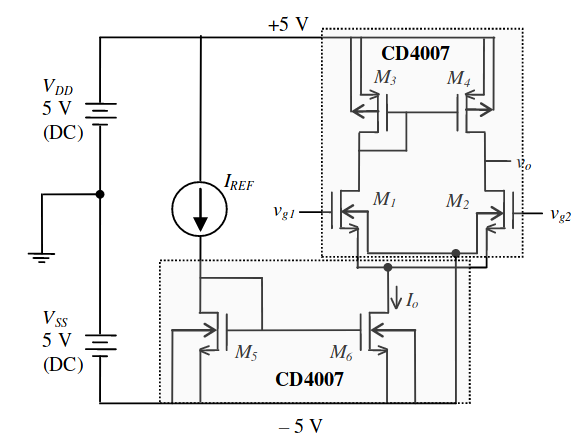
\includegraphics[width=4.0 in]{diff-amp.png}
		\caption{Differential Amplifier with current mirror load}
		\label{fig:diff-amp}
	\end{figure}

	Transistors $M_1$ and $M_2$ make up the diff-pair, $M_5$ and $M_6$
	make up the current source for the diff-pair and $M_3$ and $M_4$ are
	the load for the diff-pair. The first thing that was calculated was the 
	DC bias point for the circuit using the transistor properties and the 
	transistor current equation ($I_D = \frac{1}{2} k_n V_{ov}^2$). The values
	found for the DC bias point can be seen in Table \ref{table:qpoint}.

	\begin{table}[H]
		\centering
		\caption{DC bias point hand calculations}
		\label{table:qpoint}
		\begin{tabular}{|c|c|}
			\hline
			\textbf{Variable} & \textbf{Value}\\
			\hline
			$I$ & 4 $\si{\milli\ampere}$\\
			\hline
			$I_{D_{1,2,3,4}}$ & 2 $\si{\milli\ampere}$\\
			\hline
			$V_{GS1,2}$ & 3.3803 $\si{\volt}$\\
			\hline
		\end{tabular}
	\end{table}

	This circuit was built in PSPICE and simulated to find the bias point.
	This can be seen in Figure \ref{fig:qpoint}.

	\begin{figure}[H]
		\centering
		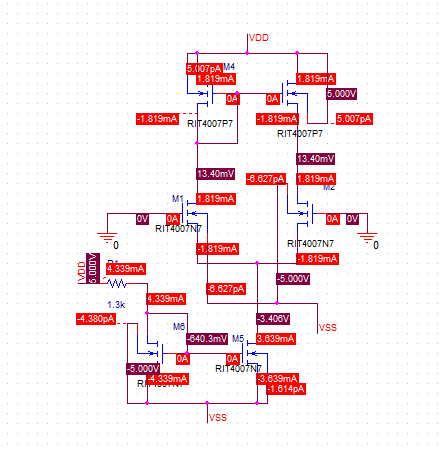
\includegraphics[width=4.5 in]{qpoint.png}
		\caption{Simulated DC bias point}
		\label{fig:qpoint}
	\end{figure}
	
	
	Another important thing to look at when building a differential amplifier is
	the differential gain. The reason that a PMOS current mirror is used as a 
	load for the diff-pair is because it effectivley doubles the double-ended 
	output gain when compared to using resistors as a load. This means that 
	the single-ended output can then be used without losing any gain. The 
	equation for this differential amplifiers single-ended gain can be seen 
	in Equation \ref{equ:diff-gain}.

	\begin{equation}
		\label{equ:diff-gain}
		A_d = gm (r_{o2} || r_{o4} || R_L)
	\end{equation}

	The differential gain that was calculated for this differential amplifier
	was 33.33 $\si\volt/\si\volt$.\\
	\hfill \break
	Another important value to look at is the common mode gain. This value shows
	how much DC input makes it to the output and can is used when calculating
	an amplifiers common mode rejection ratio (CMRR). Equation \ref{equ:cm_gain}
	shows the equation used to calculate the common mode gain and Equation
	\ref{equ:cmrr} shows the equation used to calculate CMRR.

	\begin{equation}
		\label{equ:cm_gain}
		A_{CM} = -\frac{V_o}{V_{CM}} = -\frac{1}{2g_{m_3}r_{o_3}}
	\end{equation}

	\begin{equation}
		\label{equ:cmrr}
		CMRR = \frac{A_d}{A_{CM}}
	\end{equation}

	The common mode gain for this cicruit was calculated to be 34.7
	$\si{\milli\volt}/\si\volt$. Using this value in the CMRR equation,
	a CMRR of 959.166 is found.\\
	\hfill \break
	The reason that the common mode gain matters is because, often a
	DC value has to be applied to both inputs in order to keep the 
	transistors in the circuit in saturation. In an ideal case, the
	differential amplifier would filter this out, but this value needs
	to be taken into account in order to acuratley model a real amplifier.
	Equation \ref{equ:cm_input} shows the minimum common mode voltage 
	required in order to keep all transistors in saturation.

	\begin{equation}
		\label{equ:cm_input}
		V_{CM,min} = V_{SS} + V_{GS} + V_{CS,min}
	\end{equation}

	The minimum common mode voltage required for this circuit was found
	to be 1.18 $\si\volt$.\\
	\hfill \break
	PSPICE simulations were run to find the differential and common mode
	gains. Two slightly different circuits were used to find these values
	and are shown in Figures \ref{fig:diff_gain_circuit} and 
	\ref{fig:common_gain_circuit}.

	\begin{figure}[H]
		\centering
		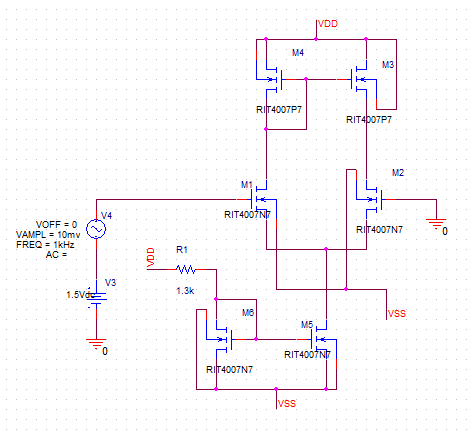
\includegraphics[width=4.0 in]{diff_gain_circuit.png}
		\caption{PSPICE circuit used to find differential gain}
		\label{fig:diff_gain_circuit}
	\end{figure}

	\begin{figure}[H]
		\centering
		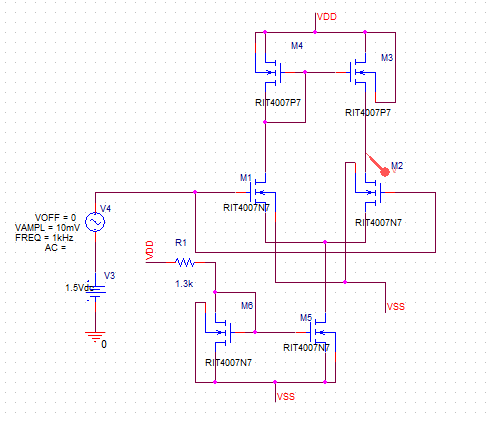
\includegraphics[width=4.0 in]{common_gain_circuit.png}
		\caption{PSPICE circuit used to find common mode gain}
		\label{fig:common_gain_circuit}
	\end{figure}

	Figures \ref{fig:pspice_diff} and \ref{fig:pspice_common} show the graph
	of the output voltage showing the peak to peak values. Since both circuits
	used inputs of 20 $\si{\milli\volt}$ peak-peak, both the differential and
	common mode gain can be calculated.

	\begin{figure}[H]
		\centering
		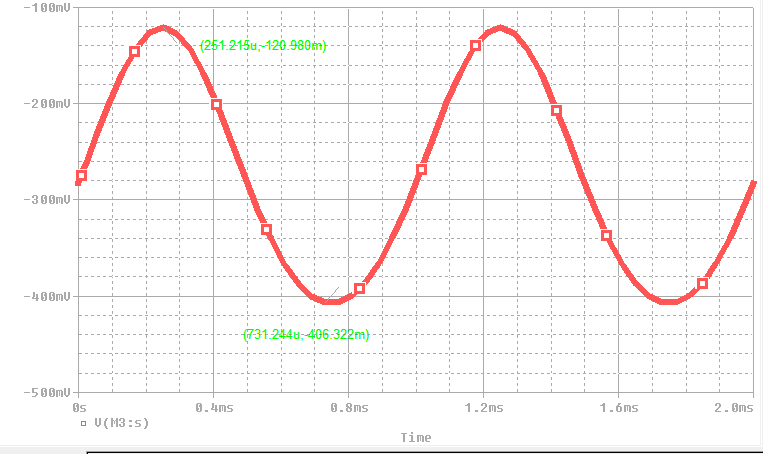
\includegraphics[width=4.0 in]{pspice_diff.png}
		\caption{PSPICE differential voltage output}
		\label{fig:pspice_diff}
	\end{figure}

	\begin{figure}[H]
		\centering
		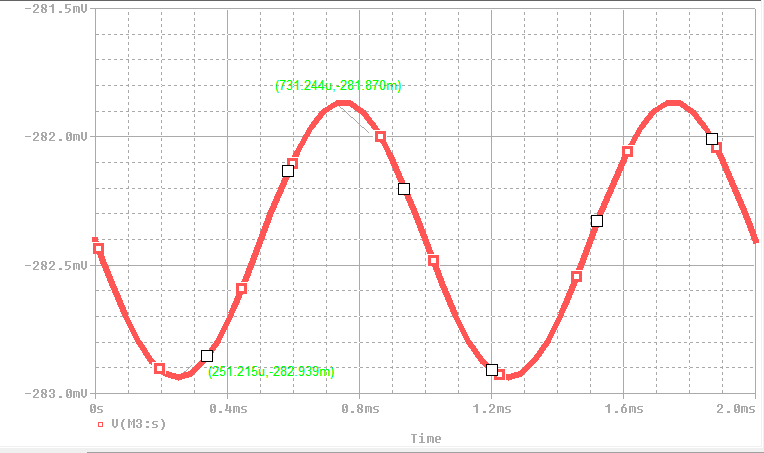
\includegraphics[width=4.0 in]{pspice_common.png}
		\caption{PSPICE common mode voltage output}
		\label{fig:pspice_common}
	\end{figure}

	Using the above graphs, the differential gain was found to be 14.27
	$\si\volt/\si\volt$ and the common mode gain was found to be 92.6
	$\si{\milli\volt}/\si\volt$. Using these two values found during simulation,
	the simulated CMRR can be calculated and was found to be 154.07.\\
	\hfill \break
	It makes sense that these values are not exactly what was calculated earlier
	beacuse the PSPICE simulation takes into acount factors like channel lenght
	modulation that the above calculations did not.\\
	
	\section{Results and Discussion}
	The next step in this lab exercise was building the circuits using two
	CD4007 packages and a breadboard. First, the current source was built
	and tested to verify that it would supply 4 $\si{\milli\ampere}$. Then the
	NMOS differential pair with PMOS current mirror load was built. \\
	\hfill \break
	The first thing that was measured was the DC bias point in order to verify
	that the circuit was properly configured. Table \ref{table:DC_exp} shows the
	DC bias point values.

	\begin{table}[H]
		\centering
		\caption{Experimental DC bias point}
		\label{table:DC_exp}
		\begin{tabular}{|c|c|}
			\hline
			\textbf{Transistor} & $V_{GS} (\si\volt)$\\
			\hline
			$Q_1$ & 3.987\\
			$Q_2$ & 3.865\\
			\hline
		\end{tabular}
	\end{table}

	The circuit was then connected to an oscilloscope and a waveform generator
	to apply input and measure the output. Just as in the simulation, two slightly
	different circuits were tested, one for the differential gain and the other 
	for the common mode gain. The scope output for both circuis can be seen in
	Figures \ref{fig:diff_gain_scope} and \ref{fig:common_gain_scope}.

	\begin{figure}[H]
		\centering
		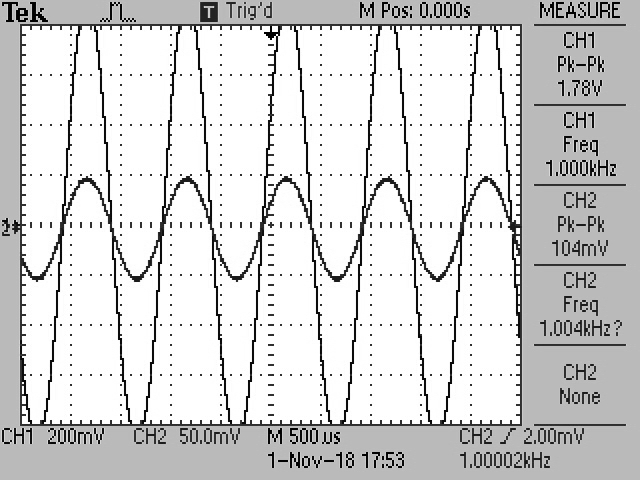
\includegraphics[width=4.0 in]{diff_gain.jpg}
		\caption{Oscilloscope differential input vs. output}
		\label{fig:diff_gain_scope}
	\end{figure}

	\begin{figure}[H]
		\centering
		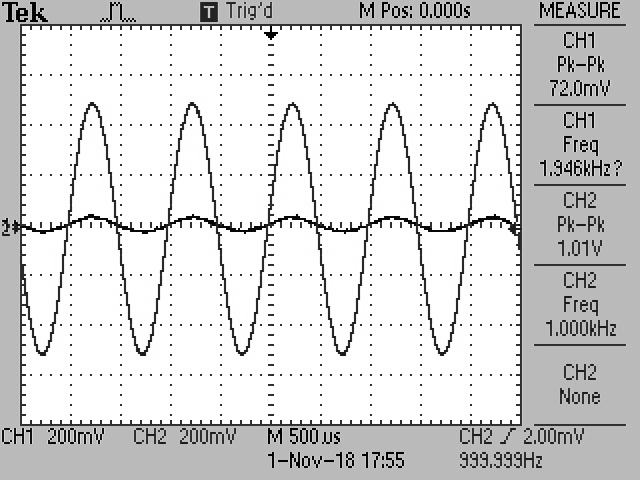
\includegraphics[width=4.0 in]{common_gain.jpg}
		\caption{Oscilloscope common mode input vs. output}
		\label{fig:common_gain_scope}
	\end{figure}

	Using the figures above, the differential and common mode gain can be 
	calculated along with the CMRR. For both figures Channel 1 shows the 
	output and Channel 2 shows input. The experimentally found values for 
	differential and common mode gain can be seen in Table 
	\ref{table:exp_gain}.

	\begin{table}[H]
		\centering
		\caption{Experimental Gain}
		\label{table:exp_gain}
		\begin{tabular}{|c|c|}
			\hline
			\textbf{Variable} & \textbf{Value}\\
			\hline
			$A_d$ & 17.12 $\si\volt/\si\volt$\\
			$A_{CM}$ & 71.29 $\si{\milli\volt}/\si\volt$\\
			CMRR & 240.09\\
			\hline
		\end{tabular}
	\end{table}
	
	Again, it makes sense that these values are slightly off from what was
	calculated and simulated, as there are effects that were not taken into 
	account during calculation or slight variations in the different transistors
	that were used in-lab. 

	Tables, graphs, equations, and prose should be used to convey all of the
	results in an easy-to-follow format. Details should be provided to 
	explain how the experimental results were obtained. The text should 
	explain any knowledge and/or information gained by performing the experiment.
	All questions posed in the labratory handout and/or by the TAs in lab should
	be answered.\\
	\hfill \break
	All plots must be created using a software package (e.g. EXCEL or MATLAB).
	Tables and equations must not be hand drawn. Be sure to include comparisions
	between theoretical, simulation, and hardware results, as well as
	comparison to design specifications where appropriate.

	\section{Conclusion}

	The goal of this lab was to build a differential amplifier using an NMOS
	simple current source (same one as Lab 3), an NMOS differential pair with
	a PMOS current mirror load. The differential amplifier was simulated and
	built in-lab and measured and compared to find the differential gain,
	common mode gain, and CMRR rating. \\
	\hfill \break
	All the values that were found during hand calculation, simulation and 
	in-lab experimentation, while they did not all match exactly, made sense
	as many of the calculations performed by hand did not take different effects
	such as channel length modulation or the body effect into account. Also
	the transistors used in-lab could have had some variability that could 
	cause them to be slightly unmatched, skewing the results.

\end{document}
